\section{Isotope labeling: tracking atoms}\label{sec:isotopes}

%\subsection{A brief history of isotope labeling and its use in electrocatalysis}

\textit{Isotope labeling} is a powerful technique to investigate mechanisms in physics, chemistry, and biology. As the name implies, isotope labeling involves intentionally preparing a material with an isotopic enrichment, and using them to keep track of how the atoms have moved around. This is in contrast to isotope geochemistry\cite{Harnung2012} and radiometric dating (including \ch{^{14}C} dating)\cite{Taylor2014, Allegre2008}, whereby the pre-existing isotopic composition of a sample is used to infer its age and origin - techniques which have provided a lot of insight into the history of earth and mankind. Whereas these techniques investigate history, isotope labeling techniques investigate how potentially useful chemical reactions take place. The former is useful in understanding the climate crisis; the latter will likely be useful in developing some of the technologies to solve it.

Here are a few interesting examples of isotope labeling experiments:
\begin{itemize}
	\item The nature of DNA replication was establishedby an isotope-labeling experiment, the Meselson - Stahl experiment\footnote{When your experiment is good enough, apparently it gets named after you. My best chance at this honor from this Thesis, though a long shot, is introduced in Subsection \ref{subsec:extraction}}, first reported in 1958, not long after the elucidation of the structure of DNA\cite{Meselson1958}. 
	
	In this experiment, E. Coli bacteria are grown in a Petri dish containing sugar and \ch{^{15}NH3}. Natural nitrogen is 99.8\% \ch{^{14}N} and 0.2\% \ch{^{15}N}, so after many generations, when these bacteria have incorporated \ch{^{15}N} in all of their nitrogen-containing molecules, including DNA, they are isotopically labeled with respect to normal E. Coli (and a bit heavier). These labeled E. Coli are then transferred to a dish containing sugar, natural \ch{NH3}, and isotopically natural versions of all of the neucleic bases that are the nitrogen-containing and information-encoding part of DNA. When these E. Coli divide, some of the DNA of the two resulting ``daughter'' cells has to be synthesized afresh. When the DNA of the daughter cells was isolated and centrifuged, it weighed exactly the average of fully labeled and non-labeled DNA! Exactly half of the nitrogen of the daughter cells was \ch{^{15}N} and half was \ch{^{14}N}. This implies that exactly one whole strand of the double-helix of each daughter cell came from the parent, and thus that DNA is replicated by the two strands unraveling and each serving as the template for a new one.
	
	\item 
	Methanol can be synthesized from syngas (\ch{CO} and \ch{H2}) on a Cu/ZnO catalyst\cite{Concepts2003} by the overall reaction
	\begin{equation}
	\ch{CO + 2 H2 -> CH3OH}\,,
	\end{equation} 
	but the reaction only runs at appreciable rates when \ch{CO2} is included in the reaction feed. \ch{^{14}C}-labeling\cite{Chinchen1987} and later \ch{^{13}C}-labeling studies\cite{Studt2015} showed that the actual methanol synthesis reaction has \ch{CO2} as the reactant:
	\begin{equation}
	\ch{CO2 + 3 H2 -> CH3OH + H2O}\,,
	\end{equation}
	and that the role of the \ch{CO} is to consume the water released and replenish the \ch{CO2} consumed by this reaction via the water-gas-shift reaction:
	\begin{equation}
	\ch{H2O + CO -> H2 + CO2}\,.
	\end{equation}
	
	\item 
	There has been a recent explosion of literature on electrochemical \ch{N2} reduction to \ch{NH3}:
	\begin{equation}
	\ch{N2 + 6 (H+ + e- ) -> 2 NH3} 
	\end{equation}
	The amounts of \ch{NH3} produced are typically very small because the reduction of water to \ch{H2} (Reaction \ref{rxn:HER2}) is almost universally favored. Nonetheless, there is an extremely sensitive colimetric technique for detection of \ch{NH3}, so many groups succeed in detecting \ch{NH3} when they run their electrochemical reaction. However, \ch{NH3} is common in the environment and it is very easy to get a false positive from \ch{NH3} contamination. Quantitative reduction of \ch{^{15}N2} to \ch{^{15}NH3}, which is easy to distinguish from \ch{^{14}NH3} using nuclear magnetic resonance (NMR), is the only accepted way to prove that the measured \ch{NH3} is formed by electrochemical \ch{N2} reduction\cite{Andersen2019}. So far, the only electrochemical strategy proven to quantitatively produce the same amount of \ch{^{15}NH3} from \ch{^{15}N2} as natural \ch{NH3} from natural \ch{N2} is an indirect one whereby lithium is reduced and then reacts with \ch{N2} to form lithium nitride which is then hydrolyzed\cite{Tsuneto1994, Andersen2019}.
\end{itemize}

Most of this Thesis will deal with Oxygen isotope labeling. Natural oxygen has three stable isotopes. On earth it is 99.76\% \ch{^{16}O}, 0.04\% \ch{^{17}O}, and 0.20\% \ch{^{18}O}\cite{Harnung2012}. There are small deviations (on the order of +/- 0.01\%) in the natural isotopic composition of oxygen on earth that are useful in isotope geochemistry, but not relevant for this Thesis. Furthermore, all of the oxygen-labeling experiments in this thesis will use natural oxygen and \ch{^{18}O}-enrichment. I will therefore only look at even masses (\ch{^{16}O2} at m/z=32, \ch{^{16}O^{18}O} at m/z=34, and \ch{^{18}O2} at m/z=36), which are unaffected by \ch{^{17}O} except for the exceedingly rare \ch{^{17}O2}. So \ch{^{17}O} is ignored throughout this thesis.

While I mentioned at the start of this Chapter that isotopes of the same element are chemically identical, this is not quite true. There are small differences, most importantly due to effect of the nuclear mass on molecular vibrational energies, that can make a small thermochemical difference between isotopes. Indeed, the most employed separation methods for almost all isotopes utilize such chemical differences (separation of \ch{^{235}U} and \ch{^{238}U} being an important exception)\cite{IsotopeSeparation}. 

The most used industrial method of separating \ch{^{18}O} from natural oxygen is by fractional distallation of \ch{NO}, as the isotope effect on the vapor pressure of \ch{NO} happens to be relatively strong\cite{Disbudak2018}. Most of the \ch{^{18}O} produced is used in the medical industry as a precursor to \ch{^{18}F} for positron emission tomography (PET).  Two commercial sources of \ch{^{18}O} are used in this Thesis: 97\% \ch{H2^{18}O} from Medical Isotopes; and 99\% \ch{^{18}O2} from \todo Where's that bottle from?

First, though, we'll take a quick look at an electrochemistry experiment in which it is instead hydrogen which is labeled. Natural hydrogen is 99.98\% \ch{^1H} and 0.02\% \ch{^2H}. The isotopes of hydrogen are important enough to get their own names, and \ch{^2H} is called \textit{deuterium} or D (such that H only refers to \ch{^1H}). \ch{D2O} is called \textit{heavy water} and is used as a non-interfering solvent in NMR, and as a neutron mediator in nuclear reactors. It is produced mainly by the Girdler-Sulfide process, which utilizes the temperature-dependence of the equilibrium constants for the reactions\cite{Agarwal2016}
\begin{equation}
\ch{H2O + HDS <-> HDO + H2S}\,\hspace{5mm}\text{and}\hspace{5mm}\ch{HDO + D2S <-> D2O + HDS}\hspace{5mm}\,.
\end{equation} 
The \ch{D2O} used in the coming experiment is from \todo Where's the \ch{D2O} from?


\subsection{Example experiment: RHE potential measurement in \ch{D2O}}\label{subsec:isotope_RHE}
As mentioned in the Foreword, I originally envisioned a short chapter called ``Hydrogen'', full of electrochemical H-D experiments, to proceed the chapter called ``Oxygen'', but ran out of time. This Subsection is a small consolation for the disappointed reader.

\begin{figure}[h!]
	\centering
	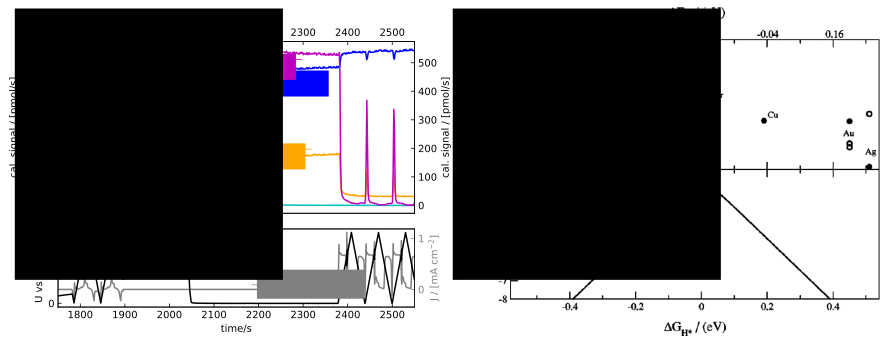
\includegraphics[width=\textwidth]{02_Tools/fig/HD_exchange.png}
	\caption{\textbf{(a)}, Electrochemical HD exchange experiment on a polycrystalline platinum electrode. The electrolyte is 0.1 M \ch{HClO4} in 99\% \ch{D2O}. Argon carrier gas is exchanged for \ch{H2} at 2050 s while the sample is at open-circuit potential, and \ch{HD} and \ch{D2} are observed (plotted on the right y-axis). \textbf{(b)}, H-D exchange current density, thus measured, for Pt (red dot) and Ir (green dot) plotted on the volcano from N\o rskov et al, 2005 (ref. \cite{Nørskov2005a}).}
	\label{fig:HD}
\end{figure}

Figure \ref{fig:HD}a shows an experiment on a polycrystalline platinum stub in deuterated electrolyte, specifically 0.1 M \ch{HClO4} in 99\% \ch{D2O}. Starting from the left, the electrode potential is cycled while in Ar-saturated electrolyte, and an m/z=4 signal is seen near the cathodic potential limit, corresponding to reduction of \ch{D2O} to \ch{D2}. It is to avoid masking the \ch{D2} signal that I use Ar (m/z=40) as the carrier gas here instead of He (m/z=4). 

The electrode potential is then set to open circuit at 1900 s, and the carrier gas is then changed from Ar to \ch{H2} at approximately 2050 s. Thus far, this is essentially the same procedure as the RHE calibration experiment demonstrated back in Subsection \ref{subsec:examples} (Figure \ref{fig:RHE_cal}). However, there is an important difference. Whereas in isotopically natural electrolyte, the HOR and HER run, undetected, at equal rates in equilibrium, now the forward and back reactions, Reactions \ref{rxn:HOR} and \ref{rxn:DER}, are distinct:
\begin{align}
\ch{H2 &-> 2 (H+ + e- )}&&\text{HOR}\label{rxn:HOR}\\
\ch{2 (D+ + e- ) &-> D2}&&\text{DER}\label{rxn:DER}
\end{align}
Thus, at the RHE condition of open-circuit voltage in 1 bar \ch{H2}, in deuterium-labeled electrolyte, there's a lot going on. The m/z=4 signal rises as \ch{H2} enters the chip, attributed to \ch{D2} from Reaction \ref{rxn:DER}. There is also a m/z=3 signal attributed to \ch{HD}. This \ch{HD} results in part from the H impurity of the electrolyte, but the \ch{HD}/\ch{D2} ratio is higher under RHE conditions than it is during reduction of the electrolyte in inert atmosphere. This indicates that some of the \ch{HD} is due to re-reduction of oxidized \ch{H2}, either via \ch{H2O} or \ch{HDO} formed by Reaction \ref{rxn:HOR} that encounters the surface of the electrode again, and/or via \ch{$*$ H} on the surface of the electrode (diagram in Figure \ref{fig:HD_diagram}). The increasing \ch{HD}/\ch{D2} ratio over the $\approx$ 5 minutes of OCV in \ch{H2}-saturated conditions indicates that at least some of it is due to \ch{H2O} or \ch{HDO}, the concentration of which would build up over time. The potential, meanwhile, falls to a steady level (-0.718 V vs the reference electrode), which is used as the zero point of the RHE potential scale even though these are not strictly equilibrium conditions.
\begin{figure}[h!]
	\centering
	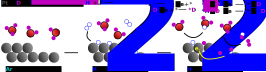
\includegraphics[width=0.75\textwidth]{02_Tools/fig/diagram_HD_exchange.png}
	\caption{Diagram indicating some of the possible surface reactions on Pt in \ch{H2}-saturated \ch{D2O} electrolyte at OCP.}
	\label{fig:HD_diagram}
\end{figure}

At about 2375 s, the potential is cycled again. Like in Figure \ref{fig:RHE_cal}a, there is an anodic current for much of the CV, where HOR is mass-transport limited. Near the cathodic potential limit of 0 V vs RHE, an m/z=4 signal reveals DER. (The cathodic potential limit in the first cycles in Ar was accidentally 10 mV anodic of the RHE potential, thus the smaller \ch{D2} signal). 

The fact that the forward and backwards reactions of the hydrogen equilibrium can be distinguished provides an interesting opportunity: this experiment can be used as a direct probe of the HER/HOR \textit{exchange current density}, which is the equal and opposite current going to the forward and backwards reactions under equilibrium. Assuming that the electrolyte at the surface of the electrode is \ch{H2} saturated, and ignoring isotope effects and the roughness of the electrode, the exchange current density is simply the DER current normalized to the electrode area:
\begin{equation}
j_0 = \frac{|I_\text{DER}|}{A_\text{el}} = \frac{2\mathcal{F}\dot{n}^{\ch{D2}}}{A_\text{el}} = \frac{2\mathcal{F}\cdot 540 \left[\frac{\text{pmol}}{\text{s}}\right]}{0.196 [\text{cm}^2]} = 0.53 \left[\frac{\text{mA}}{\text{cm}^2}\right]\,.
\end{equation} 
This exchange current density actually agrees fairly well with early reported values for the HER/HOR exchange current density on platinum\cite{Trasatti1972c, Nørskov2005a}, as shown in Figure \ref{fig:HD_diagram}a. That figure also includes the H-D exchange current density (0.55 mA/cm$^2$) measured by the same experiment on a sputterd iridium electrode.

However, there are a number of newer measurements of the exchange current density which arrive at numbers much higher than this: 120 mA/cm$^2$ for platinum nanoparticles in a Fuel-cell membrane-electrode assembly\cite{Durst2015}, $\approx$100 mA/cm$^2$ for mass-selected platinum nanoparticles in a photo-electrochemical system\cite{Kemppainen2015}, and 170-960 mA/cm$^2$ with Pt nanoparticles in a floating porous membrane interfacing the liquid electrolyte and \ch{H2} gas\cite{Zalitis2017b}. The authors of all these studies reporting very high values for the HER/HOR exchange current density claim that the earlier measurements, which typically employed rotating disk electrodes, were all measuring HER/HOR kinetics under mass transport limited conditions. Nonetheless, these old values for $j_0$ on the order of 1 mA/cm$^2$ are still often in use\cite{Tymoczko2016}.

The use of electrochemical H-D exchange to probe the exchange current density could provide a unique opportunity to resolve the issue, as it is a direct measurement of what is happening at zero net current density, the condition for which exchange current density is defined. All other studies extrapolate from non-zero current densities. However, the question is: 

\begin{question}
	Is the electrochemical H-D exchange reaction demonstrated here also mass-transport limited?\label{q:HD}
\end{question}

Figure \ref{fig:HD}a actually tells us the mass-transport limited current for HOR. It is the current in the double-layer region during the cyclic voltammagrams in \ch{H2}-saturated electrolyte, i.e., the plateau current during the cyclic voltammatry at the right in Figure \ref{fig:HD}. This current density is 0.7 mA/cm$^2$, which is more (but not a lot more) than the measured exchange current density. However, the main mass transport limitation is not actually getting \ch{H2} in, it is getting \ch{D2} out. This is because, whereas \ch{H2} can readily fill the chip and is only limited by diffusion through the working volume, \ch{D2} must not only diffuse through the working volume to the chip but must also escape the chip through the capillary. This is diagrammed in figure \ref{fig:HD_mass}a. The respective mass transport-limited current densities are:
\begin{align}
j_\text{lim}^\text{HOR} &= 2\mathcal{F} \frac{p^0}{K_H^{\ch{H2}}}\frac{D^{\ch{H2}}}{L} &= 0.67\left[\frac{\text{mA}}{\text{cm}^2}\right] \label{eq:HOR_lim}\\
j_\text{lim}^\text{DER} &= 2\mathcal{F} \frac{p^0}{K_H^{\ch{D2}}}\left(\frac{L}{D^{\ch{D2}}} + \frac{1}{h^{\ch{D2}}}\right)^{-1} &= 0.54\left[\frac{\text{mA}}{\text{cm}^2}\right] \label{eq:DER_lim}\\
\end{align}
Here, $L=100\,\mu$m is the working distance, $D^i$ is the diffusion coefficient of species $i$, $K_H^i$ is its Henry's-law constant, and $h^i$ is its mass transfer coefficient through the chip (described in Paper \ref{Trimarco2018}). I have ignored isotope effects, which are small in mass transport, and used the \ch{H2} values for \ch{D2} as well.
\begin{figure}[h!]
	\centering
	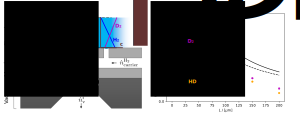
\includegraphics[width=\textwidth]{02_Tools/fig/HD_mass.png}
	\caption{Mass transport limitation in electrochemical HD exchange \textbf{(a)}, diagram of mass transport in EC-MS, indicating the \ch{H2} and \ch{D2} concentration profiles during the HD exchange experiment. \textbf{(b)}, Measured \ch{D2} and \ch{HD} fluxes, converted to partial current densities, as a function of working distance $L$. The theoretical limiting currents for HOR and DER, from Equations \ref{eq:HOR_lim} and \ref{eq:DER_lim} are included.}
	\label{fig:HD_mass}
\end{figure}

The calculated mass-transport limited current based on \ch{D2} removal from the electrode surface is remarkably close to the measured H-D exchange current density. This indicates that we, too, are just probing mass transport. The electrolyte at the surface of the electrode is thus in equilibrium, i.e. \ch{H2}, \ch{HD} and \ch{D2} follow a binomial distribution:
\begin{equation}
\frac{1}{\sum_i c^i}\begin{pmatrix}
c^{\ch{H2}}\\c^{\ch{HD}}\\c^{\ch{D2}}
\end{pmatrix}
= \begin{pmatrix}
x^2\\ 2x(1-x)\\ (1-x)^2
\end{pmatrix}\,,\hspace{1cm}\text{where}\hspace{1cm}
x \equiv \frac{c^{\ch{H+}}}{c^{\ch{D+}} + c^{\ch{H+}}}\,.
\end{equation}
One way to confirm that a reaction is mass transport limited is to establish its dependence on the working distance $L$. This can be done by exchanging the 100 $\mu$m PTFE spacer (Figure \ref{fig:chipECMS2}) with a spacer of a different thickness. Results for electrochemical H-D exchange on Pt are shown in Figure \ref{fig:HD_mass}b. While there is not a perfect match between experiment and theory, there is clearly a dependence on the apparent H-D exchange current density on distance, indicating that the answer to Question \ref{q:HD} is ``yes''.

Strategies to measure the H-D exchange current density without mass transport could include (1) doing the experiment on a sample with a small coverage of mass-selected platinum nanoparticles and/or (2) depositing the sample directly on the chip membrane, essentially setting $L=0$.

Even though this particular experiment only probed mass transport and not electrocatalytic kinetics, it indicates a promising window into the latter. Experiments avoiding mass-transport limitations by the strategies above, and testing for non-equilibrium effects on other electrocatalyst materials will follow. One particular interesting material in this regard is copper, as it shows interesting and unexpected hydrogen adsorption/desorption properties, as described in Paper \ref{Scott_Engstfeld2019}.


\subsection{Example experiment: CO stripping in \ch{H2^{18}O} electrolyte}\label{subsec:isotope_CO2}

Subsection \ref{subsec:examples} showed a CO stripping experiment on platinum, and I promised that an equivalent experiment in isotope-labeled electrolyte would come in this Section. The interesting atom to label in \ch{CO} stripping experiments is oxygen, as oxygen can have at least two origins: the \ch{CO} and the \ch{H2O} in the electrolyte.

\begin{figure}[h!]
	\centering
	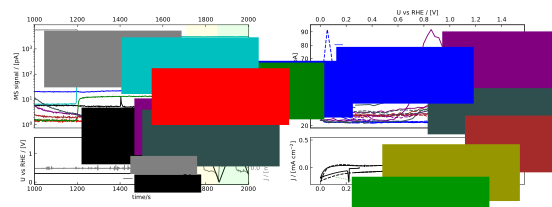
\includegraphics[width=\textwidth]{02_Tools/fig/COstrip_Ir.png}
	\caption{CO stripping experiment on a sputtered rutile \ch{IrO2} electrode in 0.1 M \ch{HClO4} in 97\% \ch{H2^{18}O}. \textbf{(a)}, as an EC-MS plot and \textbf{(b)}, plotted vs potential for the two indicated cycles. The mass spec data is raw (uncalibrated) signals.}
	\label{fig:IrO2_COstrip}
\end{figure}

Figure \ref{fig:IrO2_COstrip} shows a CO stripping experiment on a sputtered rutile \ch{IrO2} film. It is an interesting side note that crystalline \ch{IrO2} such as the sample used for Figure \ref{fig:IrO2_COstrip} adsorbs \ch{CO} at cathodic potentials, indicating that the metal atoms of the surface layer are reduced exposed; whereas electrochemically formed hydrous \ch{IrO2} does not adsorb \ch{CO}. 

From the left of Figure \ref{fig:IrO2_COstrip}a, which uses a log scale so as to include all m/z signals: the plot starts with \ch{CO} (m/z=28) as the carrier gas, and then it is switched for \ch{Ar} (m/z=40) while the electrode is held at 0.3 V vs RHE. The m/z=36 signal rises as well due to \ch{^{36}Ar}. This is actually annoying because it raises the background on \ch{^{18}O2}, a molecule of interest in \ch{^{18}O}-labeling experiments also at m/z=36. For this reason \ch{He} is used as the inert carrier gas in all subsequent \ch{^{18}O} experiments. At about 1700 s, the potential is scanned, first in the cathodic direction and then in the anodic direction. The first cycle shows some \ch{H2} (m/z=2) near the cathodic potential limit and then a number of signals on the anodic scan: m/z=46 and 44 quickly followed by 48, and then m/z=36 and 34 at the anodic limit. These are attributed to \ch{C^{16}O2} (m/z=44), \ch{C^{16}O^{18}O} (m/z=46), \ch{C^{18}O2} (m/z=48), \ch{^{16}O^{18}O} (m/z=34), and \ch{^{18}O2} (m/z=36). On the next cycle, there is more \ch{H2}, the same amount of \ch{O2}, and much less of the three isotopes of \ch{CO2}, with most of the second-cycle \ch{CO2} signal at m/z=48. The \ch{H2} and \ch{CO2} signals from these two cycles are plotted on linear scale against potential in Figure \ref{fig:IrO2_COstrip}b, showing that the \ch{CO2} signals, primarily m/z=46, start at $\approx$0.7 V vs RHE together with an anodic stripping current. 
	
\ch{CO} stripping on noble metal surfaces is believed to procede via a Langmuir-Hinshelwood mechanism\cite{Mayrhofer2005, Koper2009}, whereby adsorbed \ch{$*$ CO} reacts with adsorbed \ch{$*$ OH}. When the \ch{$*$ OH} comes from an \ch{^{18}O}-labeled electrolyte, the mechanism is:
\begin{align}
\ch{C^{16}O + $*$ &-> $*$ C^{16}O}\\
\ch{H2^{18}O + $*$ &-> $*$ ^{18}OH + (H+ + e- )}\\
\ch{ $*$ C^{16}O +  $*$ ^{18}OH &-> C^{16}O^{18}O + 2 $*$ + (H+ + e- )}
\end{align}
This implies that the \ch{CO2} desorbed should be \ch{C^{16}O^{18}O} at m/z=46. Some \ch{C^{16}O2} at m/z=44 can be expected due to the \ch{^{16}O} impurity in the electrolyte, but m/z=48 came as a huge surprise! Noble metal surfaces should not be able to split \ch{CO}\cite{Bernasek1975}!  Natural \ch{CO} is 99.8\% \ch{C^{16}O}, and I confirmed this for the \ch{CO} from our bottle by taking a mass spectrum (it is 1\% \ch{^{13}CO}, but, luckily, that can be ignored for these experiments)... I had a few fantastic days of scratching my head over this result.
\begin{figure}[h!]
	\centering
	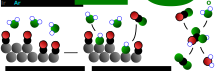
\includegraphics[width=0.6\textwidth]{02_Tools/fig/diagram_CO_strip_18O.png}
	\caption{Schematic diagram for \ch{CO} stripping in \ch{^{18}O}-labeled electrolyte (left) and subsequent homogeneous isotope scrambling via carbonic acid (right). Metal atoms are gray, carbon atoms black, hydrogen atoms white with blue outline, \ch{^{16}O} atoms red with black outline, and \ch{^{16}O} atoms are green.}
	\label{fig:diagram_CO_18O}
\end{figure}
The answer is that, while noble metal surfaces cannot split \ch{CO}, water \textit{can} split \ch{CO2}! Aqueous \ch{CO2} is in equilibrium with carbonic acid, \ch{H2CO3}. (That is, incidentally, why the oceans are getting more acidic.) The full process is indicated schematically in Figure \ref{fig:diagram_CO_18O}. The \ch{CO2} starts as \ch{C^{16}O^{18}O}, but some of it interracts with \ch{H2^{18}O} on the way out of the electrolyte and ends up switching out its \ch{^{16}O} for an \ch{^{18}O} (Reaction \ref{rxn:carbonic}).
\begin{equation}
\ch{C^{16}O^{18}O + H2^{18}O ->[$k$] H2C^{16}O^{18}O2 ->[$k$2] H2^{16}O + C^{18}O2}\label{rxn:carbonic}
\end{equation}
I actually found this very interesting, so I put some effort into exploring it. I think that the phenomenon an excellent demonstration of the world opened up by isotope studies using chip EC-MS, and so I will share with you here. CO oxidation coupled with \ch{^{18}O}-labeling will also be used in Chapter \ref{ch:O2} as a probe of lattice oxygen reactivity in oxygen evolution catalysts, so this Subsection also serves to familiarize the reader with the chemistry involved.

\begin{figure}[h!]
	\centering
	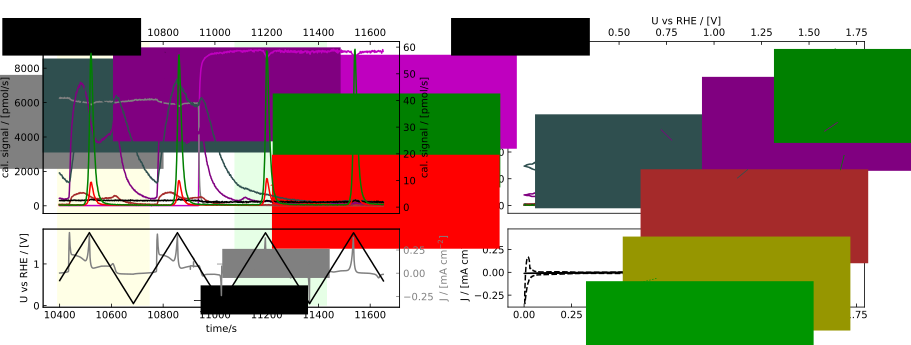
\includegraphics[width=\textwidth]{02_Tools/fig/COox_CVs_vs_potential.png}
	\caption{Cyclic voltammagrams of a polycrystalline Pt electrode in 0.1 M \ch{HClO4} in 97\% \ch{H2^{18}O}, saturated first with \ch{CO} and thereafter with \ch{He}. \textbf{(a)} As an EC-MS plot with carrier gases plotted on the left y-axis and product gases on the right y-axis. \textbf{(b)} The two cycles indicated in (a) are plotted against potential. MS signals were calibrated according to the procedures in Section \ref{sec:quantification}.}
	\label{fig:COox_CVs}
\end{figure}
One of the first things I tried was bulk \ch{CO} oxidation, akin to that in Figure \ref{fig:fig3}a. Figure \ref{fig:COox_CVs}a shows two cyclic voltammagrams of a polycrystalline \ch{Pt} electrode in CO-saturated \ch{^{18}O}-labeled electrolyte (0.1 M \ch{HClO4} in 97\% \ch{H2^{18}O}), followed by two cycles in He-saturated electrolyte. CO is oxidized to \ch{CO2} in the first two cycles, and the \ch{CO2} isotopes have distinct profiles. The \ch{C^{16}O^{18}O} profile has much sharper features and leads the \ch{C^{18}O2} profile. The origin of the features is more clear when the \ch{CO2} signals are plotted against potential, as is done in Figure \ref{fig:COox_CVs}b. 

At $\approx$ 0.9 V in the cycle in \ch{CO} (cycle 1, solid lines), an anodic peak represents the oxidative stripping of the adsorbed \ch{CO} monolayer and the depletion of \ch{CO} in the working volume on the approach to steady state. This is accompanied by a rapid increase in the \ch{C^{16}O^{18}O} signal. The current and the \ch{C^{16}O^{18}O} signal start to fall at about 1.4 V vs RHE, where the platinum surface oxidizes and loses \ch{CO} electro-oxidation activity. Then, starting at about 0.8 V vs RHE on the cathodic sweep, the sample regains some \ch{CO} oxidation activity as the surface is reduced. The gain in \ch{CO} oxidation activity outweighs the surface reduction current, but the latter is evidenced by the cathodic current at the same part of the CV in He (cycle 2). There is a corresponding peak in the \ch{C^{16}O^{18}O} signal during the cathodic scan. 

Meanwhile, the \ch{C^{18}O2} signal moves much more slowly. It increases gradually the entire anodic scan starting just after the oxidation feature at 0.9 V vs RHE, decreases only slowly during the cathodic scan, and barely registers a peak after the Pt surface is reduced. On the other hand, the \ch{C^{16}O2} signal matches the \ch{C^{16}O^{18}O} signal, just with smaller intensity.

\begin{figure}[h!]
	\centering
	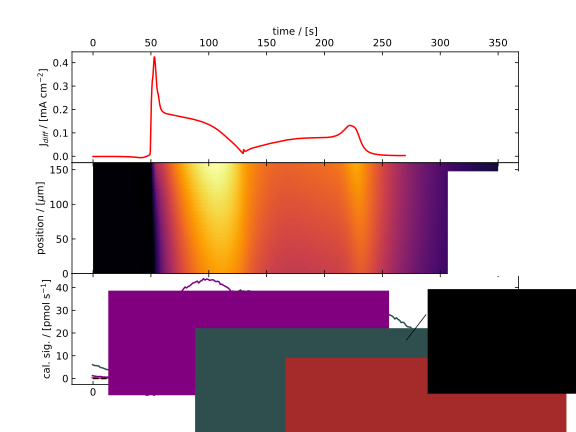
\includegraphics[width=0.75\textwidth]{02_Tools/fig/COox_CVs_predicted2.png}
	\caption{Model of \ch{CO2} signal in Figure \ref{fig:COox_CVs}. Top: CO oxidation current obtained by subtracting a cyclic voltammagram in He from a cyclic voltammagram in CO. Moddle: modeled concentration as a function of time (x axis) and distance from the membrane (y axis) in the working volume. The electrode is at the top. The working distance of $L=160\,\mu$m, indicating poor sample alignment, was determined by the mass-transport-limited \ch{CO} oxidation current. The modeled \ch{CO2} concentration varies from zero (black) to 2.2 mM (bright yellow). Bottom: the \ch{CO2} flux to the mass spectrometer predicted by the model, scaled down by a factor of 3, is co-plotted with the measured calibrated \ch{CO2} signals.}
	\label{fig:COox_pred}
\end{figure}
The question then arises:
\begin{question} 
What \textbf{should} the \ch{CO2} signal be doing?
\end{question}
This question is actually straight-forward to answer with the stagnant thin-layer model presented in Paper \ref{Trimarco2018}, which takes into account diffusion through the working volume, evaporation through the chip membrane, and removal to the vacuum chamber through the chip capillary. The input to this model is the production rate of an analyte at the electrode as a function of time. Such a production rate can be determined by subtracting the current in the cyclic voltammagram in \ch{He} (cycle 2) from the current at the corresponding time in the cyclic voltammagram in \ch{CO}. The resulting current difference is shown in the top panel of Figure \ref{fig:COox_pred}. When this is converted to a \ch{CO2} production rate assuming 2 electroons per \ch{CO2} molecule, and fed to the model, we get the concentration profile in the middle panel of Figure \ref{fig:COox_pred}. Here, the y-axis represents the position in the working volume, with the electrode on top and the chip membrane on the bottom. The predicted flux to the mass spectrometer is proportional to the calculated concentration at the chip membrane, and is shown as a dotted line in the bottom panel of Figure \ref{fig:COox_pred}. It is plotted (scaled down with a factor 3) together with the actual measured \ch{CO2} signals.

The modeled flux falls \textit{between} the \ch{C^{16}O^{18}O} and \ch{C^{18}O2} signals! In other words, while the \ch{C^{18}O2} signal is slower than expected, the \ch{C^{16}O^{18}O} signal is \textit{faster} than expected! What is going on here?

To anyone familiar with chromatography, this may seem like a separation process, whereby heavy \ch{CO2} molecules are retained longer in the working volume. However, this is getting it a bit backwards. There is no separation process - it is just that the \ch{CO2} molecules which happen to take longer to make it through the working volume are more likely to \textit{become} heavy by Reaction \ref{rxn:carbonic}. It is then a wonderful coincidence that the average time between reactions of \ch{CO2} with \ch{H2O} is on the same order of magnitude as the average time that a \ch{CO2} molecule produced at the electrode lingers in the working volume before entering the chip, and the mass spectrometer.

The actual concentration of carbonic acid (of any isotopic makeup) at any time is very small. The equilibrium constant is \cite{CRC2015}:
\begin{equation}
K_\text{eq} = \frac{c^{\ch{H2CO3}}}{c^{\ch{CO2}}} = \frac{k}{k_2} = 1.7\cdot 10^{-3}
\end{equation}
Thus, the first step in Reaction \ref{rxn:carbonic} is slow, with a rate constant $k$, and the second step is about 500 times faster. The ``wonderful coincidence'' can be stated
\begin{equation}
\tau^{\ch{CO2}}\sim\frac{1}{k}
\end{equation}
The question on my mind by this point was
\begin{question}
Based on the changes in the m/z=44, m/z=46, and m/z=48 signals, what is the rate constant $k$?
\end{question}
To answer this question in a manageable way requires having a well-defined isotope composition at $t=0$, with no additional \ch{CO2} being introduced.
\begin{figure}[h!]
	\centering
	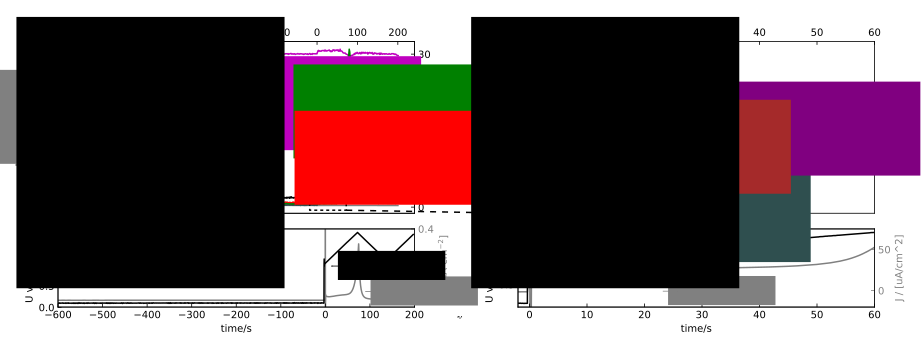
\includegraphics[width=\textwidth]{02_Tools/fig/COox_faststrip.png}
	\caption{Fast CO stripping experiment. \textbf{(a)}, The whole experiment, from when the carrier gas was switched. \textbf{(b)}, zoom-in on the \ch{CO2} signals during and right after the jump in electrode potential.}
	\label{fig:COox_faststrip}
\end{figure}
I established such a start condition by doing a ``fast \ch{CO} strip'', shown in Figure \ref{fig:COox_faststrip}. The surface of the platinum electrode is saturated with \ch{CO}, \ch{CO} is replaced by \ch{He} in the working volume electrolyte, and then, at $t=0$, the electrode potential is jumped to 1.0 V vs RHE, at which point all the \ch{CO} should immediately strip off as \ch{CO2}. Initially, there is no \ch{C^{18}O2}, as \ch{CO} does not dissociate on platinum. The \ch{C^{16}O2}-to-\ch{C^{16}O^{18}O} ratio is the same as the \ch{H2^{16}O}-to-\ch{H2^{18}O} ratio in the electrolyte (called $x$), which can be determined independently by OER, with the resulting \ch{O2} having an isotopic composition given by the binomial distribution.

To avoid worrying about the signal \ch{CO2} signal, which changes over the course of the experiment first as \ch{CO2} distributes itself in the working volume by diffusion and then as it evaporates through the chip, we just work with the normalized signals, representing the isotopic composition:
\begin{equation}
\hat{S}_\text{M44} = \frac{S_\text{M44}}{S_\text{M44} + S_\text{M46} + S_\text{M48}}\,,\hspace{1cm}\text{etc.}
\end{equation}

Given the start condition and $k$, we can write a set of differential equations relating the change in the time derivatives of $\hat{S}_M$ to the present values of $\hat{S}_M$. There are a total of eight reactions passing through a molecule of carbonic acid with mixed oxygen isotopes. These eight reactions are diagrammed in Figure \ref{fig:carbonic_kinetics}a. I've assumed that each of the three oxygen atoms of the resulting carbonic acid are equally likely to be expelled as \ch{H2O} when the new \ch{CO2} molecule is formed, resulting in the indicated probabilities.

When the effects of these eight reactions on $\hat{S}_\text{M44}$, $\hat{S}_\text{M46}$, and $\hat{S}_\text{M48}$ are added together, taking into account the activities $x$ and ($1-x$) for \ch{H2^{16}O} and \ch{H2^{18}O}, respectively, we get the following set of differential equations, shown in matrix form:
\begin{equation}
\frac{\mathrm{d}}{\mathrm{d} t} \left( \begin{array}{c}  \hat{S}_\text{M44} \\ \hat{S}_\text{M46}\\ \hat{S}_\text{M48} 
\end{array}  \right) = k \left( \begin{array}{c c c}   -\frac{2}{3}(1-x) & + \frac{1}{3}x & 0 \\  \frac{2}{3}(1-x) & -\frac{1}{3} & \frac{2}{3}x \\  0 & \frac{1}{3}(1-x) & -\frac{2}{3}x
\end{array}  \right) \left(\begin{array}{c}  \hat{S}_\text{M44} \\ \hat{S}_\text{M46}\\ \hat{S}_\text{M48} 
\end{array}  \right)
\end{equation}
And the initial condition is:
\begin{equation}
\left(\begin{array}{c}  \hat{S}_\text{M44} \\ \hat{S}_\text{M46}\\ \hat{S}_\text{M48} 
\end{array}  \right)_0 = \left(\begin{array}{c}  x \\ 1-x \\ 0 
\end{array}  \right)
\end{equation}
\begin{figure}[h!]
	\centering
	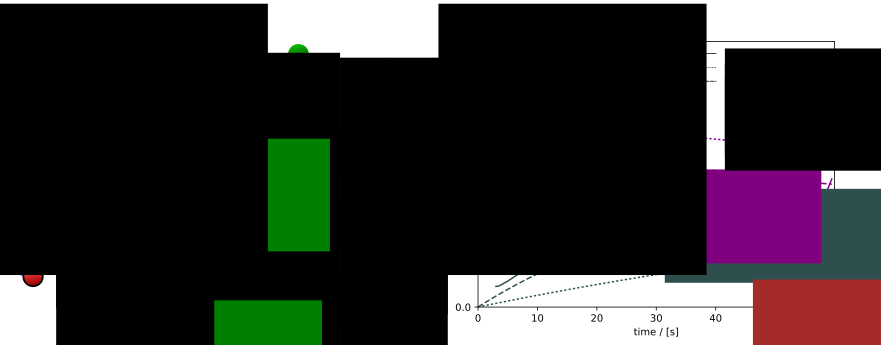
\includegraphics[width=\textwidth]{02_Tools/fig/COox_carbonic_kinetics.png}
	\caption{\textbf{(a)} Possible oxygen-exchanging reactions between \ch{H2O} and \ch{CO2}. \textbf{(b)}, \ch{CO2} isotopic compositions as a function of time from the solution of a kinetic model using two different values of the rate constant $k$ are co-plotted with the normalized measured \ch{CO2} signals from Figure \ref{fig:COox_faststrip}b}
	\label{fig:carbonic_kinetics}
\end{figure}
Numerical solution of this set of ordinary differential equations gives $\hat{S}_M$ as a function of time. The solution depends on the value of $k$. Solutions for two values of $k$ are shown in Figure \ref{fig:carbonic_kinetics}, together with the measured $\hat{S}_M$ from the experiment in Figure \ref{fig:COox_faststrip}. The first value of $k$, 0.026 s$^{-1}$, is taken from the literature\cite{Pinsent1956}. Using this value of $k$ gives a too-slow conversion of \ch{C^{16}O^{18}O} to \ch{C^{18}O2}. The second value of $k$, 0.080 s$^{-1}$, is chosen to fit the data. 

A likely cause for the discrepency is temperature: $k=0.026$ s$^{-1}$ was measured at the standard temperature of 25$^\circ$C, whereas it can easily get hotter at the sniffer setup in SurfCat's experimental hall. The actual temperature in the working volume electrolyte during that experiment could well have been 30$^\circ$C or a bit higher, which could explain the increased rate constant.

On top of being a fun opportunity to experiment with isotopes and use some differential equations, this example illustrates yet another potential application of chip EC-MS: It can in principle be used to measure the kinetics of any homogeneous reaction that:
\begin{itemize}
	\item Releases or consumes a gas (e.g. \ch{C^{18}O2})
	\item Can be triggered by either (1) an electrochemical signal (e.g. an applied potential to strip off a monolayer of \ch{CO}), or (2) introduction of a carrier gas.
\end{itemize}


\subsection{Labeling the vacuum chamber}\label{subsec:vacuum_transport}

Towards the end of the last section, I mentioned that to determine $x$, which is the fraction \ch{H2^{16}O} in the labeled electrolyte, I did so indirectly by measuring the isotopic composition of \ch{O2} produced by OER and then back-calculating $x$ from the binomial distribution. One might wonder why I didn't measure the \ch{H2^{16}O} and \ch{H2^{18}O} signals directly at m/z=18 and m/z=20, respectively. The answer is that water is notoriously ``sticky'' in vacuum chambers\cite{PfeifferKnowhow}. In effect, all of the stainless steel between the EC-MS chip and the filament acts as a chromatographic column, adsorbing water. I suspect that the stainless steel walls are normally hydroxyl-terminated, and that these hydroxyls switch out with water. My experience is that after the setup is used with \ch{H2^{18}O}, it stays ``labeled''.

\begin{figure}[h!]
	\centering
	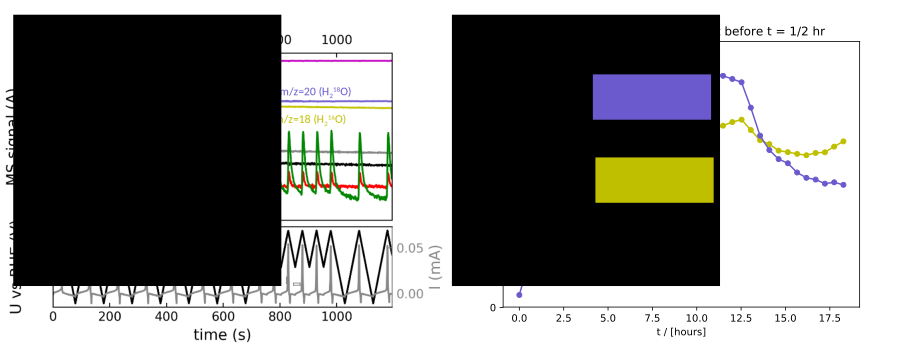
\includegraphics[width=\textwidth]{02_Tools/fig/O18_drop.png}
	\caption{\textbf{(a)}, OER experiment in \ch{^{18}O}-labeled electrolyte, showing that the m/z=18 and m/z=20 signals do not reflect the \ch{H2^{16}O} vs \ch{H2^{18}O} composition of the electrolyte. Adapted from the SI of Paper \ref{Roy2018}. \textbf{(b)}, Integrated m/z=18 and m/z=20 peaks in mass spectra taken over a 20 hour period. A drop of \ch{H2^{18}O} is applied at 0.5 hr and removed at 12.5 hr.}
	\label{fig:O18_drop}
\end{figure}
Figure \ref{fig:O18_drop}a, from the SI of Paper \ref{Roy2018}, shows cyclic voltammatry of a NiFe nanoparticle sample in 0.1 M KOH in 97\% \ch{H2^{18}O}, and includes the m/z=18 and m/z=20 signals. At the start of the experiment, these two water signals are equal, which would imply $x=0.5$.
However, the distribution of oxygen isotopes (ignoring any isotope effect) would then be
\begin{equation}
\left(\begin{array}{c}  \dot{n}_{\ch{^{16}O2}} \\  \dot{n}_{\ch{^{16}O^{18}O}}\\  \dot{n}_{\ch{^{18}O2}}
\end{array}  \right) = 
\left(\begin{array}{c}  x^2 \\ 2x(1-x) \\ (1-x)^2 \end{array}  \right) = 
\left(\begin{array}{c}  0.25 \\ 0.5 \\ 0.25 \end{array}  \right)\,,
\end{equation}
and the m/z=34 to m/z=36 ratio would be 
\begin{equation}
r = \frac{\dot{n}_{\ch{^{16}O^{18}O}}}{\dot{n}_{\ch{^{18}O2}}} = \frac{2x}{1-x} = 2
\end{equation}

In reality, the m/z=36 to m/z=34 ratio (when the signals are corrected for background) is $r=0.07$, implying (solving the above equation for $x$):
\begin{equation}
x = \frac{r}{2+r} = 0.034\,,
\end{equation}
or that the \ch{^{16}O} impurity is only 3.4\%. It would take an unrealistically powerful isotope effect to explain this discrepancy. Furthermore, the m/z=18 to m/z=20 ratio changes over the 1200 s shown, whereas the m/z=34 to m/z=36 ratio does not. Thus, the m/z=18 to m/z=20 ratio \textit{does not} represent the \ch{H2^{16}O} to \ch{H2^{18}O} ratio in the working electrolyte! Likewise, the m/z=18, 19, and 20 signals do not represent the \ch{H2O}, \ch{HDO}, and \ch{D2O} concentrations in the working electrolyte when doing H-D experiments.
\begin{question}
How long does it take to fully label the vacuum chamber? 
\end{question}
The answer is ``it depends...'', but Figure \ref{fig:O18_drop}b gives an idea. This figure shows the integral of the m/z=18 and m/z=20 peaks in mass spectra taken every 0.5 hours over the course of almost 20 hours after a drop of \ch{H2^{18}O} was placed on the EC-MS chip, covering the membrane, and left overnight under an inverted petri dish to slow its evaporation. The drop was applied after the first data point, and was removed the next morning at 12.5 hours. Surprisingly, the signals never stabilized. The m/z=20 signal reaches a peak after about 5 hours, but then starts to fall. This may indicate that the drop loses its isotopic purity by exchange with water vapor in the air. It may also have to do with the changing temperature over the course of the night. Nor does the m/z=18 to m/z=20 ratio quickly revert to normal after the drop is removed, but keeps changing for at least the duration of these measurements.
\begin{figure}[h!]
	\centering
	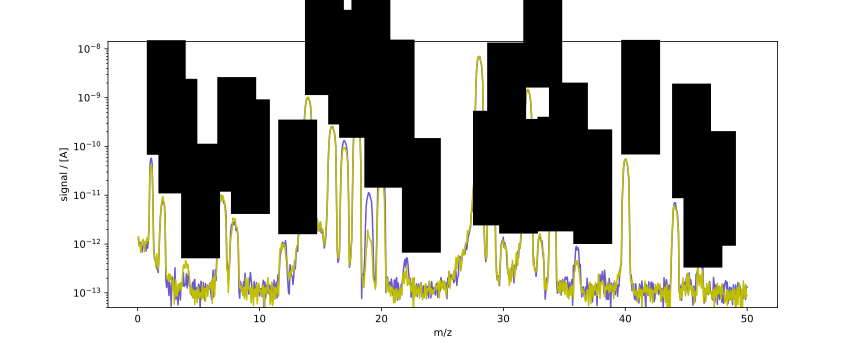
\includegraphics[width=\textwidth]{02_Tools/fig/O16_drop.png}
	\caption{Mass spectra of air through the EC-MS chip one day after experiments with \ch{^{18}O}-labeled electrolyte (purple), and after a night at 100$^\circ$C under a drop of natural \ch{H2O} (yellow). All peaks are labeled, and those in bold are related to the \ch{^{18}O} labeling of the setup.}
	\label{fig:O16_drop}
\end{figure}

Baking the vacuum chamber can help. I've found that this is especially effective if water vapor is leaked in while the chamber is heated, to speed up the removal of the \ch{^{18}O} label by switching of \ch{^{18}OH} groups for \ch{^{16}OH} groups on the stainless steel walls. Figure \ref{fig:O16_drop} shows mass spectra of air taken before and after such a baking procedure. The peaks related to \ch{^{18}O} labeling are reduced after the baking. Note that \ch{C^{18}O^{16}O} at m/z=46 is among them. However, they have not quite reached the natural ratio. Without any residual isotope labeling of the vacuum chamber, the peak at m/z=45 should be greater than at m/z=46, since \ch{^{13}C} as more than twice the natural abundance ($\approx 1$\%) of \ch{^{18}O} ($\approx 0.2$\%). This indicates that \ch{CO2} also interacts with the \ch{OH} groups on the stainless steel surfaces. 

An even more effective procedure, which does succeed in removing the \ch{C^{18}O^{16}O} is to: \textbf{Bake the chamber to 100$^\circ$C overnight under a drop of natural water with natural \ch{CO2} as the carrier gas}. 

It is very important to make sure that the vacuum chamber is not labeled before doing sensitive isotope labeling experiments such as those testing for lattice oxygen evolution described in the next Chapter. Indeed, the labeling of the vacuum chamber can even distort the apparent isotopic composition of \ch{O2} gas, as seen in the m/z=34 and especially m/z=36 peaks in Figure \ref{fig:O16_drop}.

\subsection{Other tools: Sputter deposition, ISS, and ICP-MS}\label{subsec:other_tools}

So far this chapter has exclusively described the chip EC-MS technique and its use in quantitative mass spectrometry and isotope labeling studies. Chip EC-MS has indeed been the central tool of my PhD project, but not the only one (for something completely different, see paper \ref{Scott2019_GIXRD}). This final Subsection will briefly describe a few other tools used in the next Chapter.

\textbf{Sputter deposition}

Most of the \ch{Ru}, \ch{RuO2}, \ch{Ir}, and \ch{IrO2} samples described in the next section were prepared by sputter deposition. Briefly, sputter deposition is a method of making smooth, flat thin films by physical vapor deposition, where the vapor of the desired material is formed by bombarding a target with a plasma, typically an argon plasma. This is shown schematically in Figure \ref{fig:sputter}a. 
\begin{figure}[h!]
	\centering
	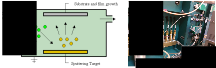
\includegraphics[width=0.8\textwidth]{02_Tools/fig/Sputtering.png}
	\caption{\textbf{(a)}, sputter deposition concept, from \url{https://en.wikipedia.org/wiki/Sputter_deposition}. \textbf{(b)} Photograph of back of our sputter chamber with \ch{^{18}O2} flask installed }
	\label{fig:sputter}
\end{figure}

The most common way to form a metal oxide by sputtering is to add \ch{O2} to the Ar used to make the plasma. This strategy is referred to as \textit{reactive sputtering}. Reactive sputtering is a simple way to prepare an isotope-labeled metal oxide sample, by switching out the natural \ch{O2} with \ch{^{18}O2}. A few months ago, I installed a small bottle of 99\% \ch{^{18}O2} on our lab's sputter chamber for this purpose (Figure \ref{fig:sputter}b). A procedure for sputtering \ch{Ru^{18}O2} and \ch{Ir^{18}O2} films is included in Appendix \ref{app:sputter}.

\textbf{Ion Scattering Spectroscopy (ISS), aka Low Energy Ion Scattering (LEIS)}

Ion scattering spectroscopy (ISS), also known as low-energy ion scattering (LEIS), is a highly surface-sensitive analysis technique based on the inelastic collisions of an ion beam, typically \ch{He+}, with a sample surface\cite{Concepts2003, Cushman2016}. This is indicated in the left of Figure \ref{fig:ISS}.

\begin{figure}[h!]
	\centering
	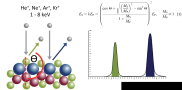
\includegraphics[width=0.8\textwidth]{02_Tools/fig/ISS_diagram.png}
	\caption{Concepts of ion scattering spectroscopy. Adapted from ref. \citen{Cushman2016} }
	\label{fig:ISS}
\end{figure}

The mechanism behind ISS is that, in such an inelastic collision, where energy and momentum are conserved, the energy of the deflected \ch{He+} ion, $E_S$, is related to the mass of the nucleus that it hits on the surface, $M_P$, according to the equation in Figure \ref{fig:ISS}. The ions are then focused, separated by energy, and detected with a \textit{hemispherical mass analyzer}. The resulting spectrum, of intensity vs deflected ion energy, then says how massive the nuclei on the sample surface that deflected the ions, are. In Figure \ref{fig:ISS}, the \ch{He+} ions (gray) would deflect off of the large surface atoms (blue) with a greater energy than the small surface atoms (green), as the latter would recoil more on collision. This gives rise to two the green and blue peaks, respectively.

ISS is especially useful in the context of this thesis because, since it probes the nuclei of the sample rather than its electronic structure, it is isotope sensitive. ISS is therefore the tool to answer the following question, which becomes important in the latter parts of Chapter \ref{ch:O2}:
\begin{question}
Is the oxygen at the surface of my metal oxide sample \ch{^{16}O} or \ch{^{18}O}?
\end{question}

All of the ISS spectra presented in Section \ref{sec:lattice_O} were taken by Jakob Ejler using the Omicron setup. I took all of the ISS spectra presented in Section \ref{sec:dissolving} using the Thetaprobe setup after Ezra Clark got it working.


\textbf{Inductively Coupled Plasma - Mass Spectrometry (ICP-MS)}

As described in the start of the next Chapter, stability is an important issue in electrocatalysis, especially oxygen evolution in acid, which requires rare and expensive iridium- and/or ruthenium-based electrocatalysts. Under these conditions, most materials dissolve, and even the best materials dissolve slowly.

The question, as it has been phrased by Cherevko and coworkers\cite{Geiger2018}, is:
\begin{question}
	How many molecules of product, on average, does one atom of element \textbf{i} in the electrode make before it is lost?
\end{question}
The answer to this question, called the \textit{stability number}, is also called the \textit{turn-over number} in conventional catalyst. The stability number depends on both the electrode material and the conditions, including the electrode potential.

Determining the stability number is best done by measuring the concentration of the metal of interest ($i$) in the electrolyte. The most sensitive way to measure a small concentration of metal ions is inductively-coupled plasma mass spectrometry (ICP-MS)\cite{Harris2010, Frydendal2014}.
\begin{figure}[h!]
	\centering
	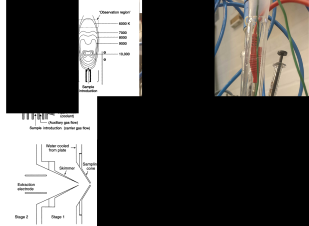
\includegraphics[width=0.8\textwidth]{02_Tools/fig/ICPMS_diagrams.png}
	\caption{\textbf{(a)} Diagram of inductively-coupled plasma (ICP) torch (top) and its coupling to mass spectrometer (bottom). Adapted from ref. \citen{Gross2007}. Figure numbers in the image refer to that textbook. \textbf{(b)} Photo of setup for taking electrolyte samples during EC-MS experiments for dissolution analysis by ICP-MS. (The carrier gas inlet volume was going through a bit of a transition phase.) }
	\label{fig:ICPMS}
\end{figure}
In ICP-MS, the MS part is basically the same as that described in the start of Section \ref{sec:ECMS} - a quadrupole mass analyzer is typically used for mass separation and detection. The unique part in ICP-MS is the inlet and ionization\cite{Gross2007}, with diagrams shown in Figure \ref{fig:ICPMS}a. This is done by directly delivering the liquid to a plasma torch, which has an extremely hot argon plasma formed by magnetic induction from external magnetic coils. The plasma is hot enough to atomize the liquid, and the plasma delivers electric charges to any metal atoms that were dissolved in the liquid. These metal ions are then separated from the non-ionized parts of the plasma by lenses through two pumping stages and delivered mass spectrometer. ICP-MS is an extremely sensitive technique, able to detect on the order of parts per trillion (nanograms per liter) of metals in solution.

Most of the work involved in ICP-MS, for the experimenter, is preparing the samples. I came up with a way to collect electrolyte from the stagnant thin-layer EC-MS cell during an experiment without losing potential control using the setup shown in Figure \ref{fig:ICPMS}a. See Appendix \ref{app:sampling} for detailed instructions on how to take electrolyte samples using this setup. Briefly, the electrolyte in the cell is sucked out with a syringe while new electrolyte flows in from an electrolyte delivery tower. The old electrolyte stored in an Eppendorf tube and the syringe is re-inserted. This results in electrolyte samples of $\approx 0.5$ ml in Eppendorf tubes. 

For study with ICP-MS, the raw samples are first diluted to a standard volume of 1 ml with 2\% \ch{HNO3}, 0.1 ml of this is then diluted to 10 ml with 2\% \ch{HNO3}, which is the ICP-MS sample. The concentration of this ICP-MS sample is then as if all of the metal dissolved during the experiment were diluted in 100 ml. The amount of metal $n^i$ (typically stated in pmol) can then be determined from its mass concentration $c_m^i$ in the ICP-MS sample (typically stated in $\mu$g per l which is numerically equivalent to ppb) by
\begin{equation}
n^i = 100\,\text{[ml]}\frac{c_m^i}{M^i}\,,\label{eq:ppb_to_pmol}
\end{equation}
where $M^i$ is the molar mass of $i$.

To determine $c_m^i$ from the raw signal (in counts) requires calibration. A dilution series (typically 0.1, 1, 10, and 100 $\mu$g/l) is prepared from a standard stock solution. These are measured together with the samples and intervening measurements a blank solution (2\% \ch{HNO3} in water with no metals). The calibration curve is made by drawing a line of best fit through the counts vs concentrations of this dilution series on a log-log plot (the slope of this line should be 1). Typical calibration curves for Ir and Ru are shown in Figure \ref{fig:ICPMS_cal}. These calibration curves are made using the function \texttt{ICPMS\_calibration} of the \texttt{EC\_MS} python package (see Appendix \ref{app:EC_MS}).

\begin{figure}[h!]
	\centering
	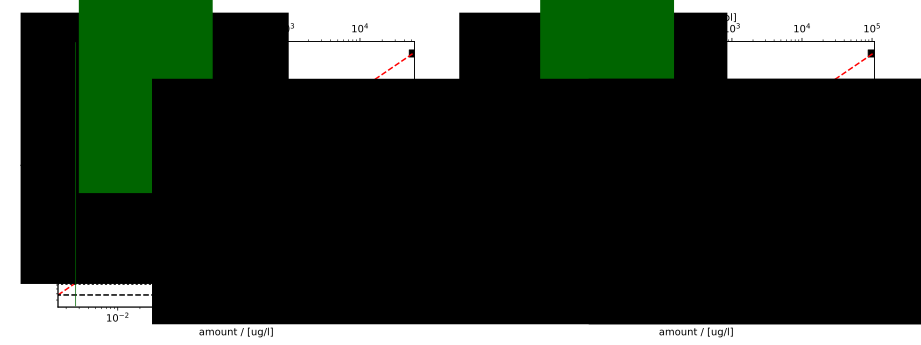
\includegraphics[width=\textwidth]{02_Tools/fig/ICPMS_calibration_curves.png}
	\caption{Calibration curves for ICP-MS detection of \textbf{(a)} Ir and \textbf{(b)} Ru. The top x-axes represents the amount of metal originally in a sample from the EC-MS setup, and is scaled to the bottom x-axis according to Equation \ref{eq:ppb_to_pmol}. The dashed black line is the mean number of counts in blank measurements, and the dotted black line is that mean plus three times the standard deviation of the number of counts in the blank measurement. The detection limit, defined as where the latter intercepts the calibration curve, is indicated with a green vertical line.}
	\label{fig:ICPMS_cal}
\end{figure}

The detection limit is defined as the amount corresponding to the counts of the blank measurements plus three times the standard deviation of counts the blank measurements\cite{Harris2010}. This is 1.4 pmol for Ir and 3.1 pmol for Ru.

\textbf{Concluding remark:}

This concludes the chapter on the tools used in this PhD project, the principle one of which is chip EC-MS, to which I view the data analysis package \texttt{EC\_MS} as an essential extension. Together with isotope labeling, it often feels as if chip EC-MS opens a window to the world of electrocatalysis from a new and mostly unexplored angle. It is often easier to freely explore this world than to step back and ask controlled and disciplined questions. I will do my best at the latter in the next Chapter, but I hope that this Chapter has given a sense of the thrill of the exploration that I have been enjoying for most of the past three years.
